% 124-18(124쪽) — $y=a\cos bx+c$ 의 그래프. 최댓값·최솟값 자리의 가로 점선($2$, $-6$), $x=8$ 에서 꼭짓점으로 내린 세로 점선,
% 축 아래 라벨 $8$ 까지 원문 그대로.
% 스캔 화질이 낮아 TikZ 로 다시 그림. 원문에 없는 눈금·$a$, $b$, $c$ 의 값은 넣지 않는다.
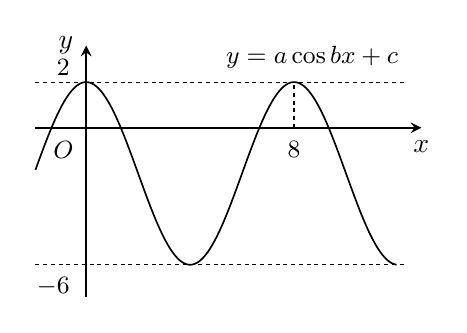
\begin{tikzpicture}[line width=0.6pt, x=0.33cm, y=0.29cm]
  \draw[dashed, dash pattern=on 1.4pt off 1.4pt, line width=0.4pt] (-1.95,2) -- (12.35,2);
  \draw[dashed, dash pattern=on 1.4pt off 1.4pt, line width=0.4pt] (-1.95,-6) -- (12.35,-6);
  \draw[dashed, dash pattern=on 1.4pt off 1.4pt, line width=0.4pt] (8,0) -- (8,2);
  \draw[->, >=stealth, line width=0.7pt] (-1.95,0) -- (12.9,0) node[below=1pt] {$x$};
  \draw[->, >=stealth, line width=0.7pt] (0,-7.4) -- (0,3.6) node[left=1pt] {$y$};
  \draw[domain=-1.95:11.95, samples=200, smooth] plot (\x, {4*cos(45*\x)-2});
  \node[anchor=south east, font=\small] at (-0.25,1.85) {$2$};
  \node[anchor=north east, font=\small] at (-0.25,-6.1) {$-6$};
  \node[anchor=north east, font=\small] at (-0.1,-0.15) {$\pt{O}$};
  \node[anchor=north, font=\small] at (8,-0.15) {$8$};
  \node[anchor=south west, font=\small] at (5.0,2.15) {$y=a\cos bx+c$};
\end{tikzpicture}
